% !TeX spellcheck = fr_FR
\chapter{Chapitre 7 : Base de données et données persistantes}

\section*{Pourquoi un chapitre sur la base de données ?}

Cette application est construite autour d'un \textit{graphe spatial} de points d'arrêt provenant de plusieurs mondes: ATLAS (référentiel officiel), OpenStreetMap (OSM), GTFS et HRDF pour les lignes. Le rendu cartographique en temps réel, l'analyse des problèmes et la consolidation des correspondances s'appuient sur un schéma de base de données optimisé pour la lecture, avec une logique d'\textit{ingestion} explicite. 

Ce chapitre rend cette mécanique visible, avec des extraits de code, des schémas, et des graphiques générés directement depuis la base existante.

\vspace{0.5em}
\textbf{Spoiler} — le chapitre \texttt{chap8.tex} plongera ensuite dans le backend (API, endpoints, sécurité, pagination, etc.), en s'appuyant sur les éléments que nous posons ici.

\section{Importer les données: le rôle de \texttt{import\_data\_db.py}}
L'import est orchestré par le script \texttt{import\_data\_db.py}. Il ne se contente pas d'insérer des lignes: il nettoie, croise des sources, calcule des priorités de problèmes, et construit des artefacts prêts pour l'interface.

\subsection*{Vue d'ensemble}
\begin{codebox}[language=Python]{Pipeline d'import des données}
build_route_direction_mapping()  # cartographie GTFS/OSM/HRDF -> (route, direction) <-> (noeuds, SLOIDs)
load_route_data()                # routes par SLOID (ATLAS) et par node_id (OSM)
load_unified_route_data()        # vue unifiée (gtfs/hrdf) par SLOID
import_to_database(...)          # insère stops, détails ATLAS/OSM, routes, problèmes
apply_persistent_solutions()     # réapplique les solutions/notes persistantes
\end{codebox}

L'import crée des \textit{stops} de trois types:\ \texttt{matched} (paires ATLAS–OSM), \texttt{unmatched} (ATLAS isolé), \texttt{osm} (OSM isolé). Les détails riches (ex: opérateur ATLAS, tags OSM, routes) sont stockés dans des tables dédiées afin que le rendu des \emph{popups} reste instantané et autonome.

\subsection*{Un extrait révélateur}
Pour la ré-application des données persistantes, le script balaye la table \texttt{persistent\_data} et met à jour les nouveaux enregistrements:

\begin{codebox}[language=Python]{Ré-application des solutions persistantes}
# Extrait de import_data_db.py -> apply_persistent_solutions()
persistent_solutions = session.query(PersistentData)\
    .filter(PersistentData.note_type.is_(None)).all()

for ps in persistent_solutions:
    matching_stops = session.query(Stop)\
        .filter((Stop.sloid == ps.sloid) | (Stop.osm_node_id == ps.osm_node_id))\
        .all()
    
    for stop in matching_stops:
        problem = session.query(Problem).filter(
            Problem.stop_id == stop.id,
            Problem.problem_type == ps.problem_type
        ).first()
        
        if problem:
            problem.solution = ps.solution
            problem.is_persistent = True
\end{codebox}

\paragraph{Important} Nous n'exécutons pas l'import dans ce chapitre (la base est déjà peuplée). Les statistiques et graphiques ci-dessous proviennent d'un script d'analyse dédié (\S\ref{subsec:scripts-ch7}).

\section{Schéma logique: les tables qui comptent}

Le schéma applicatif est défini dans \texttt{backend/models.py}. Voici les entités principales:

\begin{description}
  \item[\texttt{stops}] Table centrale pour le rendu cartographique. Colonnes clefs: \texttt{sloid}, \texttt{stop\_type}, \texttt{match\_type}, coordonnées (\texttt{atlas\_lat/lon} et \texttt{osm\_lat/lon}), \texttt{distance\_m}, \texttt{osm\_node\_type}, \texttt{atlas\_duplicate\_sloid}.
  
  \item[\texttt{atlas\_stops}] Détails ATLAS par \texttt{sloid}: désignation, opérateur, routes unifiées, notes persistantes.
  
  \item[\texttt{osm\_nodes}] Détails OSM par \texttt{osm\_node\_id}: tags de transport, opérateur, routes OSM, notes.
  
  \item[\texttt{problems}] Détections automatiques (\texttt{distance}, \texttt{unmatched}, \texttt{attributes}, \texttt{duplicates}), solution éventuelle, \texttt{priority} et traçabilité auteur.
  
  \item[\texttt{persistent\_data}] Stockage des solutions et notes destinées à survivre aux ré-imports.
  
  \item[\texttt{routes\_and\_directions}] Consolidation GTFS/HRDF/OSM par (\texttt{route\_id}, \texttt{direction\_id}) ou (\texttt{line\_name}, \texttt{direction\_uic}).
\end{description}

\subsection*{Diagramme conceptuel}

\begin{codebox}{Schéma relationnel des tables principales}
+-------------------+             +---------------------+
|   atlas_stops     |<----------->|      stops          |
|  (sloid PK)       |    sloid    | (id PK)             |
+-------------------+             | sloid, osm_node_id  |
                                  | atlas_*  osm_*      |
+-------------------+    osm_id   | distance_m          |
|    osm_nodes      |<----------->| stop_type, ...      |
|(osm_node_id PK)   |             +---------------------+
+-------------------+                        |
                                             | stop_id
+-------------------+              +---------v-----------+
|    problems       |<-------------|      stops          |
| (stop_id FK)      |              | (id PK)             |
+-------------------+              +---------------------+

+--------------------------+
|    persistent_data       |     <- Solutions/notes persistantes
| (sloid, osm_node_id,     |        entre re-imports
|  problem_type, note_*)   |
+--------------------------+

+--------------------------+
| routes_and_directions    |     <- Consolidation GTFS/HRDF/OSM
|  (route_id, direction)   |        pour filtres UI
+--------------------------+
\end{codebox}

\noindent
Remarque: les liens \og stops → détails \fg{} sont réalisés par \textit{jointures explicites} (\texttt{sloid}, \texttt{osm\_node\_id}) plutôt que des clés étrangères rigides. Ce choix facilite l'ingestion et limite les verrouillages lors des rafraîchissements, tout en gardant des \textit{indexes} ciblés pour les requêtes critiques.

\subsection*{Index utiles pour la carte}
\begin{itemize}
  \item \texttt{idx\_atlas\_lat\_lon} et \texttt{idx\_osm\_lat\_lon} pour filtrer vite par fenêtre cartographique.
  \item \texttt{idx\_stop\_type\_match\_type} pour les filtres dynamiques.
  \item \texttt{idx\_distance\_m} pour les tris par distance.
  \item Sur \texttt{routes\_and\_directions}: \texttt{idx\_osm\_route\_direction}, \texttt{idx\_atlas\_route\_direction}, \texttt{idx\_atlas\_line\_direction\_uic}.
\end{itemize}

\section{Pros et cons du schéma vis-à-vis du rendu cartographique}
\subsection*{Points forts}
\begin{itemize}
  \item \textbf{Lecture optimisée}: une ligne de \texttt{stops} suffit pour dessiner un marqueur (ATLAS ou OSM) sans \texttt{JOIN}.
  \item \textbf{SARGable viewport}: la requête de fenêtre cartographique est \emph{sélective} grâce aux index lat/lon des deux mondes (extrait d'API ci-dessous).
  \item \textbf{Détails séparés}: les tables \texttt{atlas\_stops} et \texttt{osm\_nodes} chargent les popups à la demande (lazy) sans gonfler la ligne \texttt{stops}.
  \item \textbf{Routes consolidées}: la table \texttt{routes\_and\_directions} alimente les filtres par ligne et direction côté UI.
\end{itemize}

\subsection*{Compromis}
\begin{itemize}
  \item \textbf{Intégrité logique}: l'absence de FK strictes suppose une discipline d'import (gérée par \texttt{import\_data\_db.py}).
  \item \textbf{Duplication contrôlée}: certaines valeurs (ex: \texttt{distance\_m}) sont redondantes par design pour éviter des calculs à la volée.
  \item \textbf{Évolution des tags OSM}: les champs \texttt{osm\_*} sont \textit{snapshottés}; toute évolution nécessite un nouvel import.
\end{itemize}

\subsection*{La requête de fenêtre}

\begin{codebox}[language=Python]{Filtrage géographique optimisé — backend/blueprints/data.py}
# Requête SARGable pour l'endpoint /api/data
viewport_sargable = or_(
    # Points ATLAS dans la fenêtre
    and_(Stop.atlas_lat.between(min_lat, max_lat),
         Stop.atlas_lon.between(min_lon, max_lon)),
    
    # Points OSM seuls dans la fenêtre  
    and_(Stop.atlas_lat.is_(None), Stop.atlas_lon.is_(None),
         Stop.osm_lat.between(min_lat, max_lat),
         Stop.osm_lon.between(min_lon, max_lon))
)

query = query.filter(viewport_sargable)
\end{codebox}

\section{Statistiques et graphiques depuis la base}
Tous les chiffres et graphiques ci-dessous proviennent d'une interrogation \textit{en lecture seule} de la base existante (aucun ré-import ou recalcul global). Comme mentionné au \textbf{chapitre 5}, l'analyse de contenu et l'interprétation détaillée ont déjà été présentées; nous évitons ici de nous répéter et nous référons à ce chapitre pour la discussion approfondie. Nous nous concentrons ici sur la \textit{fraîcheur des chiffres} et leur \textit{usage pour l'architecture}.

\subsection{Volumes globaux}
Comme mentionné au \textbf{chapitre 5}, nous avions présenté ces ordres de grandeur. Ici, nous donnons les \textit{totaux actualisés} issus de la base au moment de la génération (\S\ref{subsec:scripts-ch7}):\\
\texttt{77\,074} entrées dans \texttt{stops}, dont \texttt{48\,528} \texttt{matched}, \texttt{9\,537} \texttt{unmatched} (ATLAS isolés) et \texttt{19\,009} \texttt{osm} (OSM isolés).

\begin{figure}[h]
  \centering
  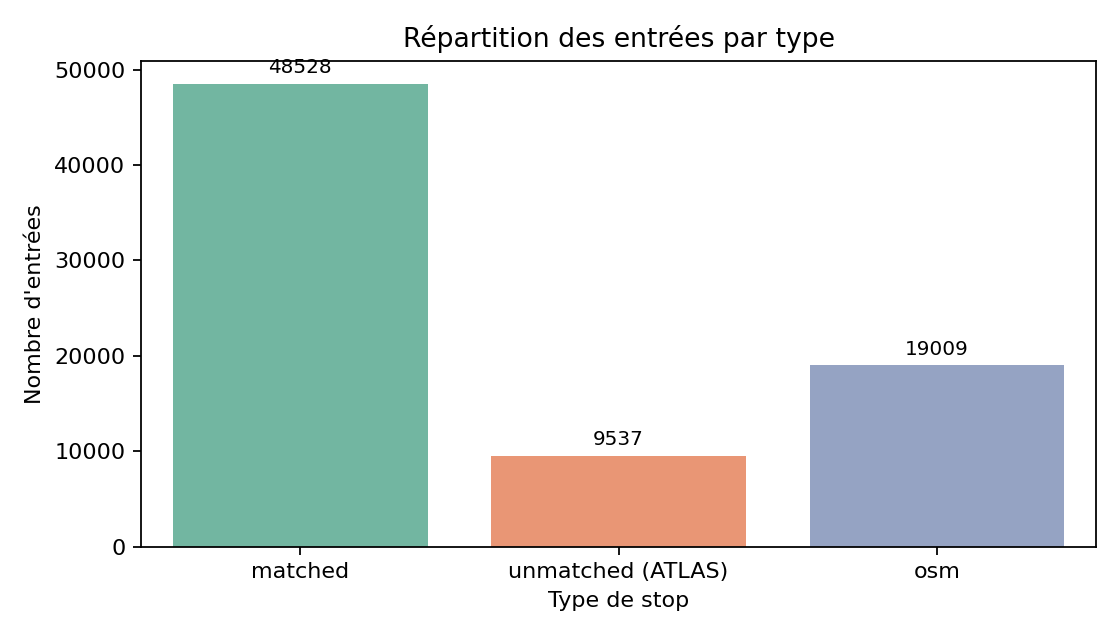
\includegraphics[width=0.68\linewidth]{figures/chap7/stops_by_type.png}
  \caption{Répartition des entrées par type (lecture directe de \texttt{stops}).}
\end{figure}

\subsection{Distances des correspondances}
Comme mentionné au \textbf{chapitre 5}, la distribution des distances ATLAS–OSM présente un cœur près de 0–20 m et une queue longue. Nous mettons simplement à jour la \textit{photographie} ci-dessous provenant de la base actuelle.

\begin{figure}[h]
  \centering
  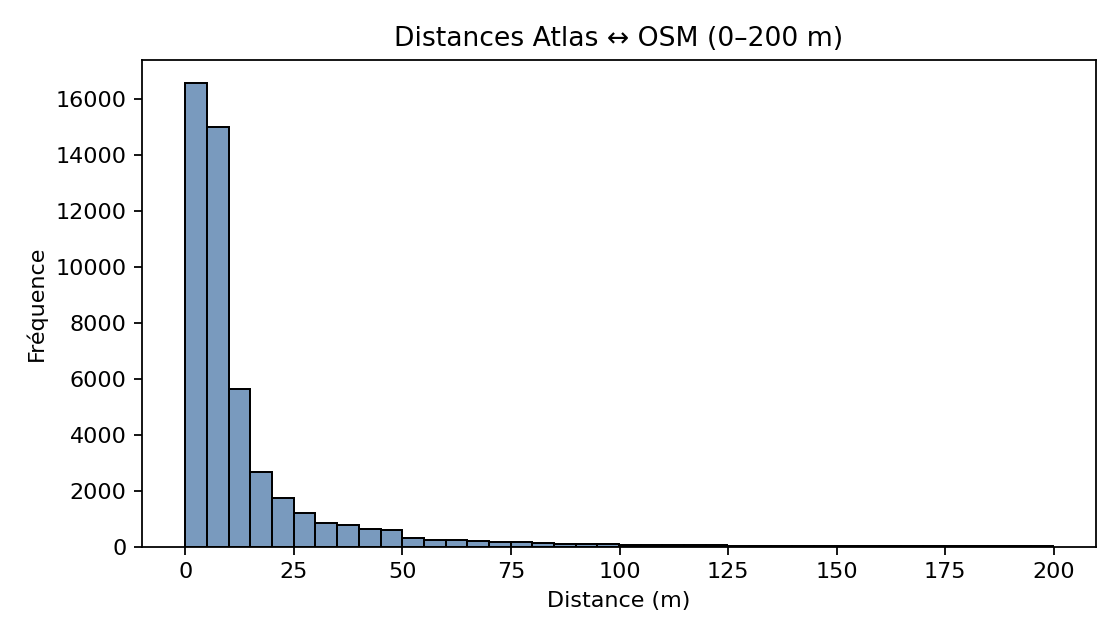
\includegraphics[width=0.68\linewidth]{figures/chap7/distances_hist_0_200.png}
  \caption{Histogramme des distances ATLAS–OSM entre 0 et 200 m (mise à jour).}
\end{figure}

\begin{figure}[h]
  \centering
  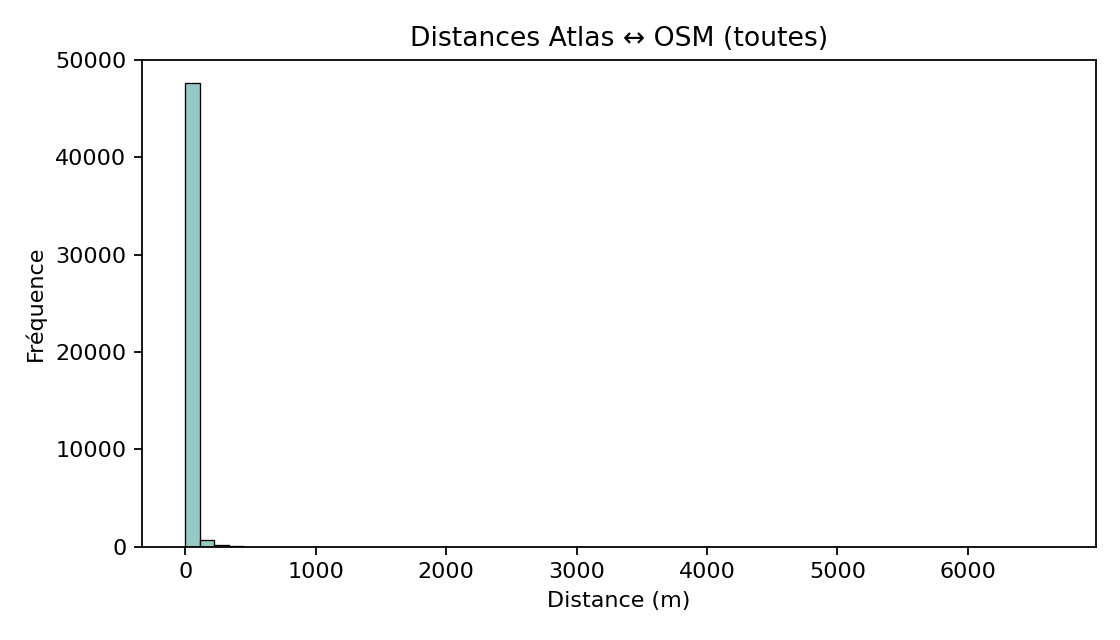
\includegraphics[width=0.68\linewidth]{figures/chap7/distances_hist_all.png}
  \caption{Histogramme des distances ATLAS–OSM (toutes distances, mise à jour).}
\end{figure}

\subsection{Problèmes détectés}
Comme mentionné au \textbf{chapitre 5}, les familles dominantes sont \texttt{distance}, \texttt{unmatched} et \texttt{attributes}. Ci-dessous, un \textit{état actualisé} utile pour la priorisation dans l'interface (nous renvoyons à l'analyse du chapitre 5 pour les conclusions).

\begin{figure}[h]
  \centering
  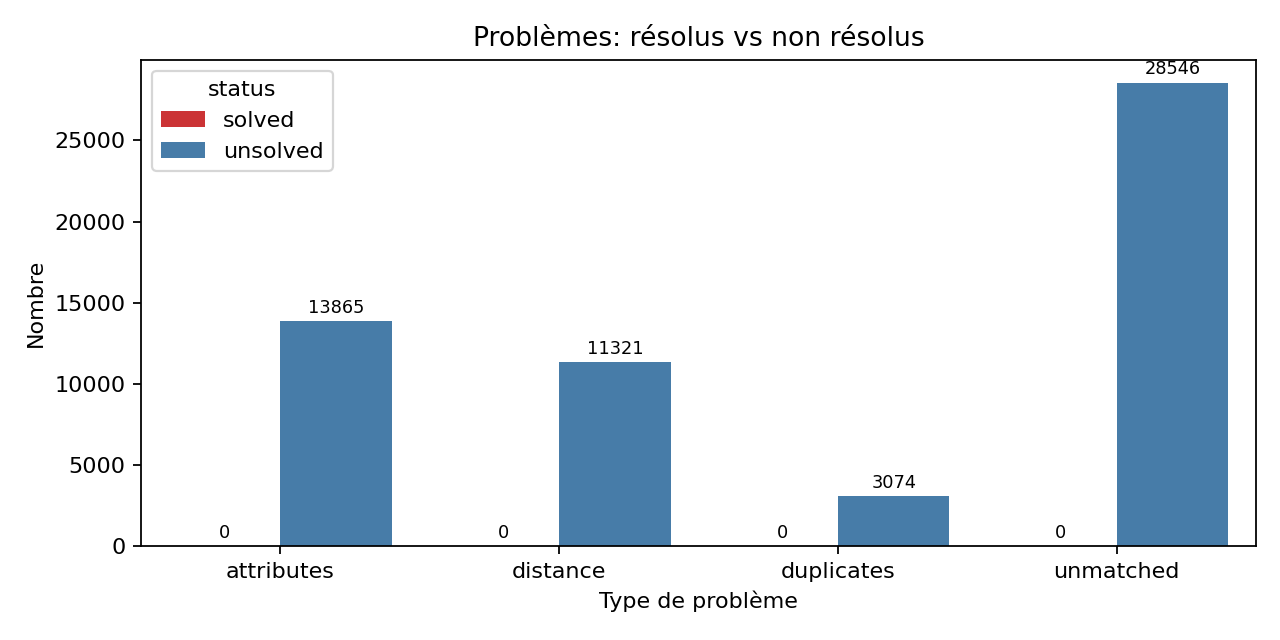
\includegraphics[width=0.75\linewidth]{figures/chap7/problems_breakdown.png}
  \caption{Problèmes: résolus vs non résolus, par type (état actualisé).}
\end{figure}

\subsection{Routes et directions}
Comme mentionné au \textbf{chapitre 5}, nous avons déjà décrit les familles \texttt{matched} / \texttt{osm\_only} / \texttt{atlas\_only}. Ci-dessous, la vue consolidée (GTFS/HRDF) \textit{mise à jour} qui alimente les filtres côté UI.

\begin{figure}[h]
  \centering
  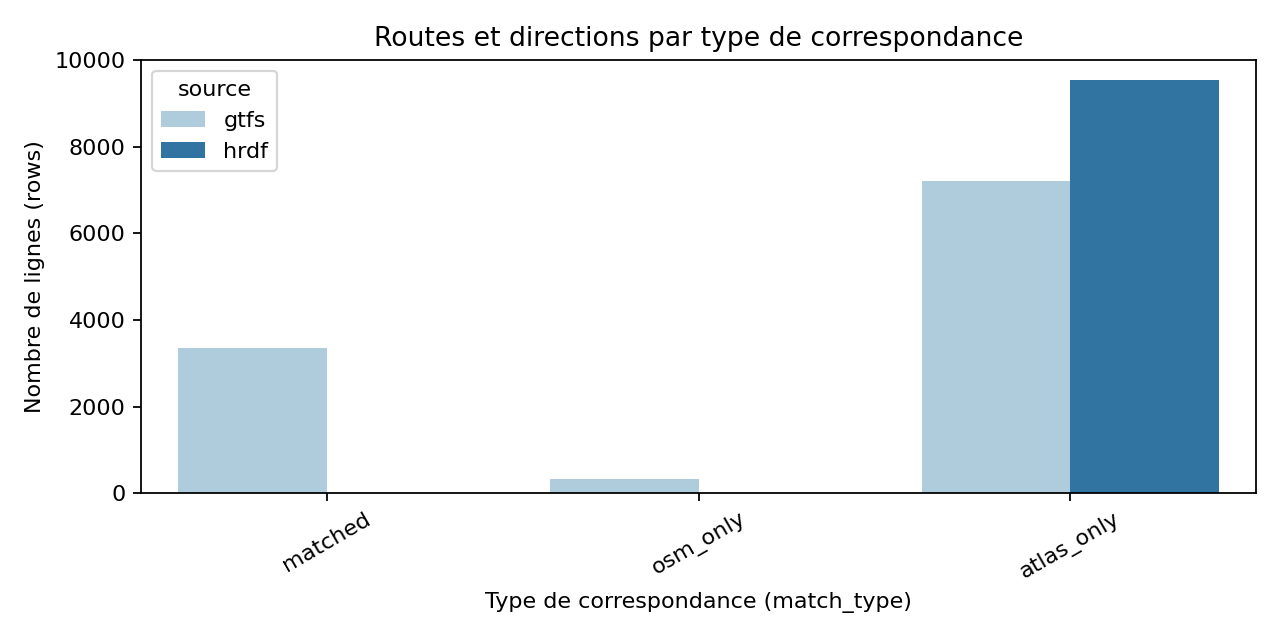
\includegraphics[width=0.80\linewidth]{figures/chap7/routes_match_breakdown.png}
  \caption{Routes/directions par type de correspondance (GTFS et HRDF, mise à jour).}
\end{figure}

\section{Données persistantes: comment elles survivent aux ré-imports}
Le mécanisme de persistance se trouve à deux endroits:\ (i) l'API de gestion (\texttt{/api/make\_solution\_persistent}, \texttt{/api/save\_note/...}),\ (ii) l'étape \texttt{apply\_persistent\_solutions()} de l'import.

\subsection*{Côté base}
La table \texttt{persistent\_data} stocke:
\begin{itemize}
  \item des \textbf{solutions} par triplet \texttt{(sloid, osm\_node\_id, problem\_type)};
  \item des \textbf{notes} persistantes côté ATLAS (\texttt{note\_type = 'atlas'}) ou OSM (\texttt{'osm'}).
\end{itemize}

\subsection*{Côté web (UI)}
Dans l'interface \og Problèmes \fg{}, l'utilisateur peut:
\begin{itemize}
  \item résoudre un problème, puis \textit{rendre la solution persistante} (bouton dédié) ;
  \item saisir une note côté ATLAS ou OSM et la marquer persistante ;
  \item effectuer un \textit{match manuel} entre deux entrées (ATLAS $\leftrightarrow$ OSM) et l'enregistrer de manière durable.
\end{itemize}
Nous ajouterons des captures d'écran de l'interface dans une version ultérieure du manuscrit.

\subsection*{Un mini-exemple côté navigateur}

\begin{codebox}{Match manuel persistant — interface web}
// Extrait simplifié de la logique JS de match manuel
$.ajax({
    url: '/api/manual_match',
    method: 'POST',
    contentType: 'application/json',
    data: JSON.stringify({
        atlas_stop_id: atlasId,
        osm_stop_id: osmId,
        make_persistent: true
    }),
    success: function(response) {
        console.log('Match persistant créé:', response);
    }
});
\end{codebox}

\noindent
Lors du prochain import, la solution manuelle réapparaîtra \textit{sans effort} grâce à \texttt{apply\_persistent\_solutions()}.

\section{Performance: pourquoi ça défile vite sur la carte}

L'expérience utilisateur fluide de la carte interactive repose sur deux ingrédients architecturaux clés:

\begin{description}
  \item[Ligne auto-suffisante pour le rendu] La table \texttt{stops} contient toutes les informations nécessaires au rendu d'un marqueur. Un \textit{viewport query} n'a pas besoin de joindre des tables lourdes: la position et la nature du marqueur (\texttt{osm\_node\_type}) sont \og en main \fg{}.
  
  \item[Index spatiaux ciblés] Les clauses \texttt{BETWEEN} sur les coordonnées (\texttt{atlas\_lat/lon}, \texttt{osm\_lat/lon}) exploitent des index dédiés, permettant une sélection très rapide par fenêtre géographique.
\end{description}

\paragraph{Chargement différé des détails} Les informations riches (opérateur, routes, notes) sont chargées \textit{au clic} pour construire les popups — ce qui évite de surcharger la phase de \textit{fetch} initial. Cette stratégie de \textit{lazy loading} maintient des temps de réponse constants même avec des milliers de points.

\paragraph{Optimisations côté client} Les marqueurs qui se superposent géographiquement sont \og décalés \fg{} de quelques pixels afin de rester individuellement cliquables, sans impact sur les performances de rendu.

\section{Scripts utilisés et reproductibilité}
\label{subsec:scripts-ch7}
Tous les chiffres et figures ont été produits par le script ci-dessous, que vous trouverez dans \texttt{memoire/scripts\_used/chap7/db\_overview.py}. Il interroge la base en lecture seule et enregistre les images sous \texttt{memoire/figures/chap7/}.

\begin{codebox}[language=bash]{Génération des statistiques et graphiques}
python3 memoire/scripts_used/chap7/db_overview.py
\end{codebox}

\noindent
Les figures insérées dans ce chapitre sont: 
\texttt{stops\_by\_type.png}, \texttt{distances\_hist\_0\_200.png}, \texttt{distances\_hist\_all.png}, \texttt{problems\_breakdown.png}, \texttt{routes\_match\_breakdown.png}.

\section{Réflexion et pistes d'amélioration}
\textbf{Qualité des données}. Une partie de la queue longue des distances provient d'objets OSM de type \texttt{stop\_position} éloignés. Une heuristique fine par opérateur (tram/bus/rail) pourrait réduire ces écarts.

\textbf{Intégrité et évolutivité}. Introduire des contraintes souples (\textit{deferred constraints} ou validateurs applicatifs) pour détecter les \og orphelins \fg{} si un détail ATLAS/OSM est manquant.

\textbf{Routes unifiées}. Poursuivre la normalisation des \texttt{route\_id} (ex. neutralisation des suffixes \texttt{-j24}) pour renforcer la jointure \texttt{gtfs $\leftrightarrow$ atlas} déjà amorcée par la fonction de normalisation.

\textbf{Indexation spatiale}. Tester une indexation géospatiale (MySQL SRID 4326 ou PostGIS si migration) pour accélérer encore les fenêtres sur de très grands jeux.

\textbf{Cache côté API}. Mettre en cache les réponses de petites fenêtres urbaines très fréquentées (ex: centre-ville) avec invalidation lors d'un nouvel import.

\textbf{Traçabilité des matches manuels}. Ajouter un historique horodaté des matches/notes avec l'auteur pour faciliter les audits.

\section*{Et ensuite ?}
Le \textbf{Chapitre 8} sera consacré au backend: architecture des blueprints, endpoints clés (\texttt{/api/data}, \texttt{/api/problems}, \texttt{/api/operators}, etc.), sécurité (authentification, 2FA), pagination, et \og règles de politesse \fg{} vis-à-vis du SGBD. Nous y disséquerons les stratégies de requêtage et d'optimisation mises en place.




